\chapter*{Travail réalisé}
\addcontentsline{toc}{chapter}{Travail réalisé}
\setcounter{section}{0} % Réinitialisation du compteur de section

\section{Technologies utilisées}

\begin{center}
    \begin{minipage}{\textwidth}
        \begin{minipage}{0.2\textwidth}
            \centering
            
\includegraphics[width=1\textwidth]{images/logo/angular.jpeg}
        \end{minipage}\hfill
        \begin{minipage}{0.75\textwidth}
            \textbf{Angular} est un framework de développement frontend avec une structure modulaire. Permet de créer des applications web de type SPA (Single page application) dynamiques et robustes.
        \end{minipage}
    \end{minipage}

    \vspace{2em} % Espace entre les figures

    \begin{minipage}{\textwidth}
        \begin{minipage}{0.2\textwidth}
            \centering
            
\includegraphics[width=0.5\textwidth]{images/logo/springBoot.png}
        \end{minipage}\hfill
        \begin{minipage}{0.75\textwidth}
            \textbf{Spring Boot 3} est un framework Java open source, un framework de développement backend, pour simplifier et accélérer le développement d'application Java.
        \end{minipage}
    \end{minipage}


    \vspace{2em} % Espace entre les figures
    
    \begin{minipage}{\textwidth}
        \begin{minipage}{0.2\textwidth}
            \centering
            
\includegraphics[width=0.4\textwidth]{images/logo/typeScript.png}
        \end{minipage}\hfill
        \begin{minipage}{0.75\textwidth}
            \textbf{TypeScript} est un sur-ensemble du langage JavaScript dont j'ai eu l'occasion de découvrir lors de mon parcours universitaire, ajoutant de nouvelles fonctionnalités et syntaxes.
        \end{minipage}
    \end{minipage}

    \vspace{2em} % Espace entre les figures
    
    \begin{minipage}{\textwidth}
        \begin{minipage}{0.2\textwidth}
            \centering
            
\includegraphics[width=0.5\textwidth]{images/logo/postgres.svg.png}
        \end{minipage}\hfill
        \begin{minipage}{0.75\textwidth}
            \textbf{PostgreSQL} est un système de gestion de base de données relationnelles. On a choisi cette base car l'entreprise a privilégié de migrer toutes ses applications sur PostgreSQL, car les licences Oracle deviennent plus chères.
        \end{minipage}
    \end{minipage}

    \vspace{2em} % Espace entre les figures
    
    \begin{minipage}{\textwidth}
        \begin{minipage}{0.2\textwidth}
            \centering
            
\includegraphics[width=0.5\textwidth]{images/logo/ittelij.jpg}
        \end{minipage}\hfill
        \begin{minipage}{0.75\textwidth}
            \textbf{IntelliJ IDEA 2024.1} comme environnement de développement de l'application.
        \end{minipage}
    \end{minipage}

    \vspace{2em} % Espace entre les figures
    
    \begin{minipage}{\textwidth}
        \begin{minipage}{0.2\textwidth}
            \centering
            
\includegraphics[width=0.35\textwidth]{images/logo/flyway.png}
        \end{minipage}\hfill
        \begin{minipage}{0.75\textwidth}
            \textbf{Flyway} est un outil de migration de base de données qui permet de gérer et d’automatiser les versions des schémas de base de données de manière cohérente.
        \end{minipage}
    \end{minipage}

    \vspace{2em} % Espace entre les figures
    
    \begin{minipage}{\textwidth}
        \begin{minipage}{0.2\textwidth}
            \centering
            
\includegraphics[width=0.5\textwidth]{images/logo/maven.png}
        \end{minipage}\hfill
        \begin{minipage}{0.75\textwidth}
            \textbf{Maven} est un outil de gestion de la construction de logiciels. Il aide à compiler et tester un logiciels, mais aussi à le distribuer et à le rendre simple à comprendre par d'autres développeurs.
        \end{minipage}
    \end{minipage}
\end{center}

\newpage

\section{Architecture}
Dans le cadre de mon stage, j'ai eu l'occasion d'explorer la dynamique entre les différentes technologies utilisées. L'architecture du projet se schématise de la façon suivante :
\medskip

\begin{figure}[h!]
    \centering
    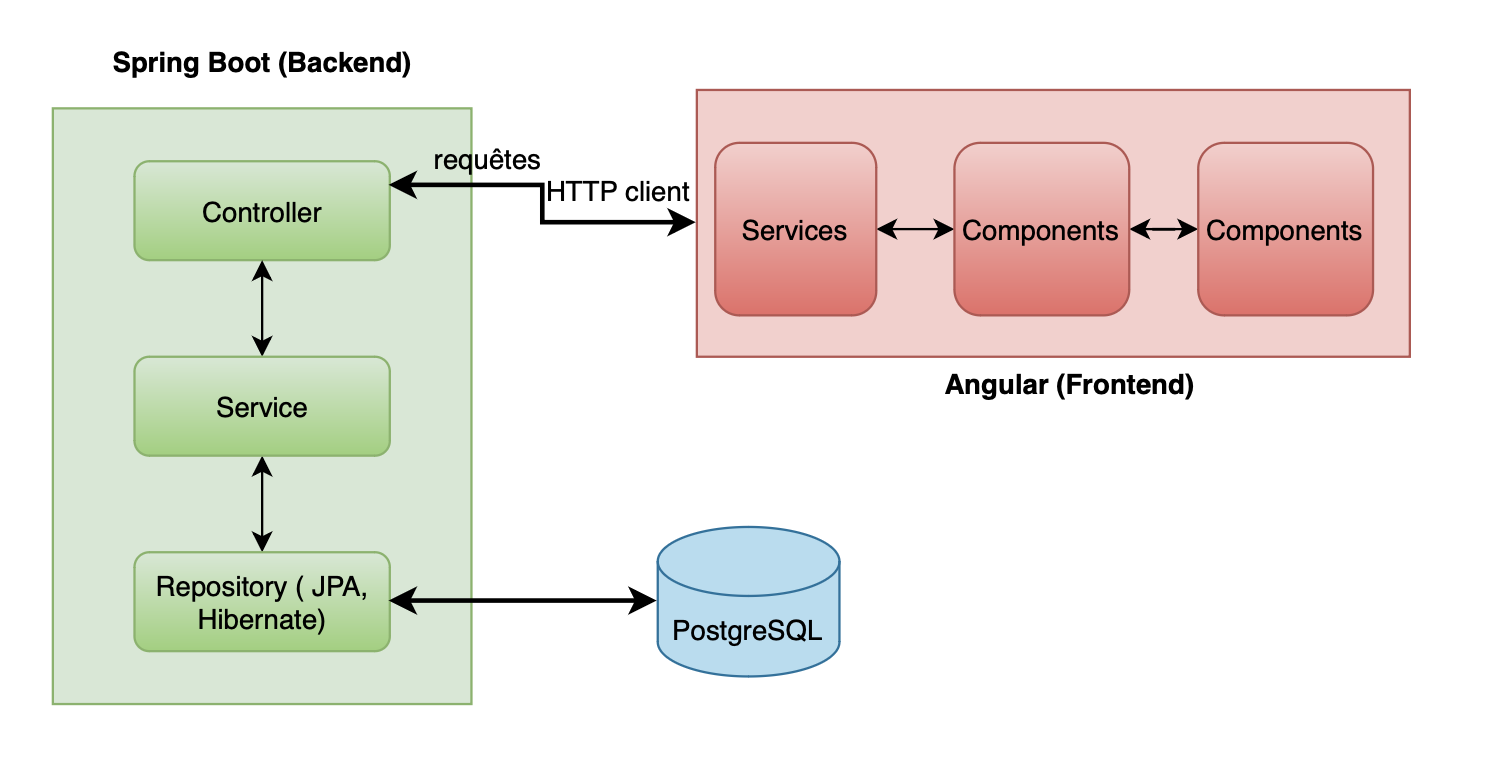
\includegraphics[width=0.8\textwidth]{images/diagramme/archi.png}
    \caption{Architecture de l'application}
\end{figure}
\medskip

Cette représentation illustre la manière dont les différentes technologies interagissent entre elles. Les éléments qui participent à l'interaction entre l'utilisateur, l'application et la base de données sont le 'Controller', le 'Service' et le 'Repository'. Chacun ayant un rôle spécifique :
\medskip

Controller : gère les interactions entre l'utilisateur et l'application, agissant comme un pont entre l'utilisateur et l'application. Il reçoit et traite les requêtes de l'utilisateur et dirige les actions appropriées vers les services correspondants.
\medskip

Service : implémente les traitements nécessaires pour répondre aux demandes de l'utilisateur. il interagit avec les 'Repository' pour accéder aux données. 
\medskip

Repository : gère l'interaction avec la base de données, il utilise JPA, un framework ORM, pour mettre en pratique le patrons de conception DAO pour exécuter des requêtes SQL sans avoir besoin de les écrire. Cette approche facilite la communication avec la source de données.
\medskip

\subsection{Mise en place}
Concernant la mise en place du projet, nous avons suivi les étapes suivantes :
\medskip

\textbf{Mise en place de la stack et configuration de l'environnement de développement} : Nous avons débuté par la création d'un dépot Git pour la gestion collaborative du code source, suivi de la configuration de la structure du projet et de son environnement à l'aide de Docker. Docker nous permet de créer des images systèmes adaptées à nos besoins, tandis que NGINX a été utilisé comme serveur pour exposer les services de notre application Angular.
\medskip

Une fois l'image construite elle sera hébergée, déployée sur Kubernetes, qui est un orchestrateur qui permet de gérer les images dockers, permet de déployer des services. Kubernetes va lancer l'image et exécuter le fichier 'entrypoint.sh' qui démarre notre service Angular avec la commande  `ng serve`.
\medskip

\textbf{Création des squellettes backend et frontend :} Nous avons utilisé les outils Spring Initializr et Angular CLI pour générer les squellettes de nos projets backend et frontend respectivement. En personnalisant ensuite les configurations de base pour le projet Anguler. Cette approche nous a permis de démarrer rapidement le développement.
\medskip

    \subsection{Partie frontend}
    Le développement a débuté par la mise en place de l'interface utilisateur qui repose sur le framework Angular. Les composants ont été créés progressivement en fonction des exigences fonctionnels de l'application. Cela a permis de prendre en mains le framework Angular et de comprendre comment il fonctionnait.
    \medskip

    L'application est divisée en plusieurs composants qui intéragissent avec les services, dont la figure ci-dessous illustre les différents composants :
    \medskip

    \begin{figure}[h!]
        \centering
        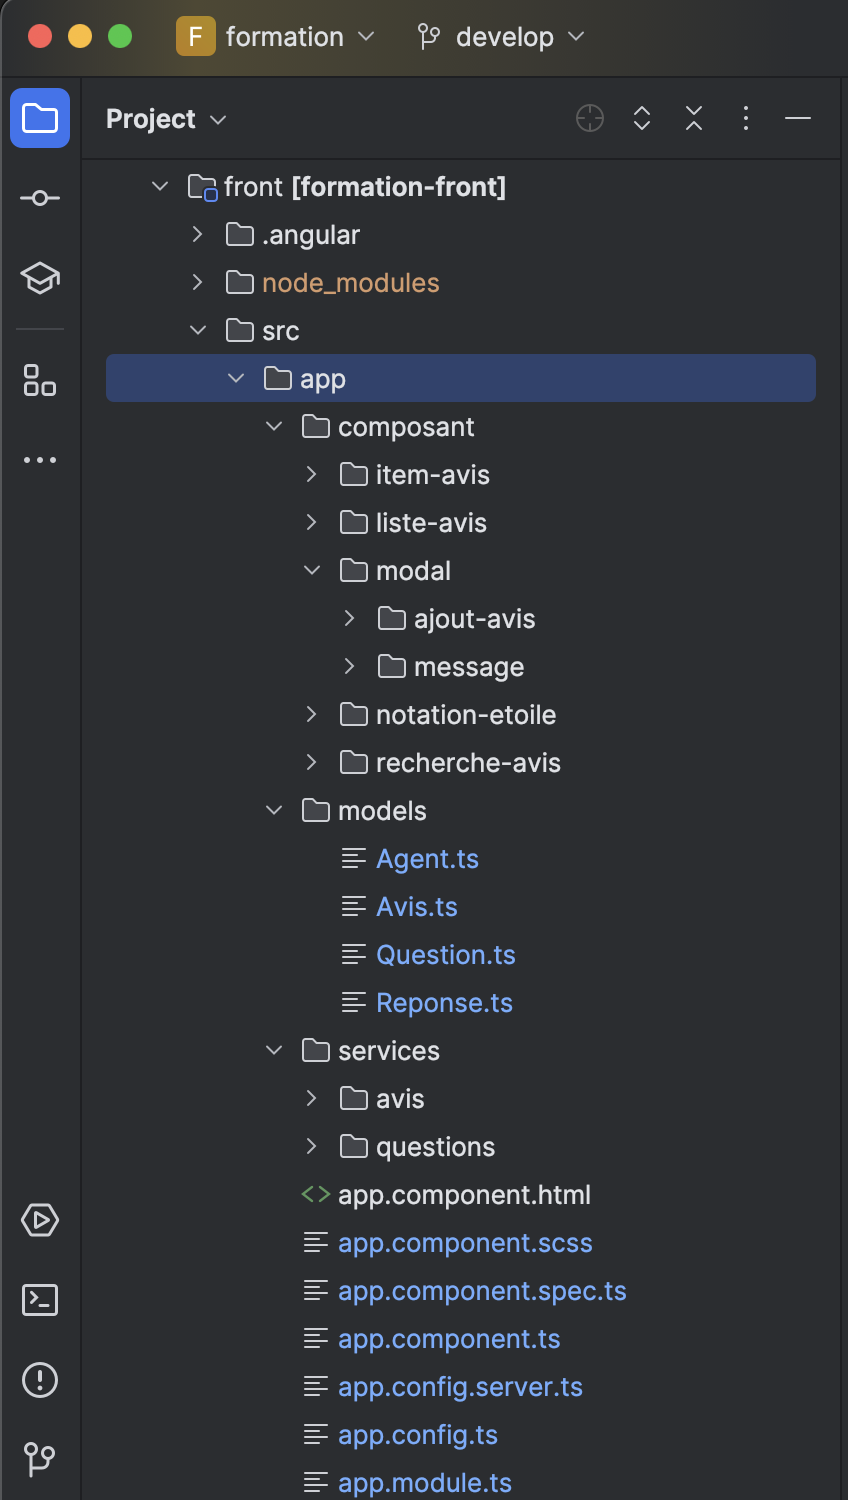
\includegraphics[width=0.5\textwidth]{images/code/composant.png}
        \caption{Les différents composants de l'application}
    \end{figure}
    \medskip

    Les différents composants sont les suivants :
    \medskip

    \begin{itemize}
        \item Le composant ajout-avis, qui représente une fenêtre modale permettant l'affichage du formulaire de création ou affichage de l'avis.
        \item Le composant liste-avis, qui représente la page web principale pour l'affichage de la liste des avis.
        \item Le composant item-avis, qui représente chaque item d'un avis, chacun composé d'une note et d'un commentaire.
        \item Le composant notation-etoile, qui représente un système de notation par étoiles.
        \item Le composant recherche-avis, qui représente le composant de la barre de recherche d'un avis.
        \item Le composant message, qui permet la gestion des notifications.
    \end{itemize}
    \vspace{0.5cm}

    Deux services sont utlisés dans l'application pour gérer les opérations communes entre les composants.  Ces services ont le rôle de pont entre les composants et les appels HTTP à l'API backend de l'application.    
    \medskip

    Le service avis a les fonctionnalités suivantes :
    \medskip
    
    \begin{itemize}
        \item Récuperer tous les avis : cette fonctionnalité permet de récuperer les avis à partir de l'API backend en envoyant une requête HTTP GET.
        \item Ajouter un avis : cette fonctionnalité permet d'ajouter un avis en envoyant une requête HTTP POST à l'API backend pour ajouter l'avis dans la base de données.
        \item Chercher un avis : cette fonctionnalité permet de chercher un avis à partir d'une information spécifique en envoyant une requête HTTP GET à l'API backend.
    \end{itemize}
    \medskip

    Le service question a la fonctionnalité suivante :\medskip
    \begin{itemize}
        \item Récuperer toutes les questions : cette fonctionnalité permet de récuperer les questions du formulaire de notation à partir de l'API backend en envoyant une requêtes HTTP GET.
    \end{itemize}\medskip
    
    \subsection{Partie backend}
    Avant de commencer l'implémentation de la partie back, il est crucial de définir clairement notre modèle de données et les interactions utilisateurs via des diagrammes UML. Ces représentations graphiques nous permettent de visualiser et de structurer la solution objet de manière claire et précise. 
    \medskip
    \subsubsection{2.2.1\hspace{2em}Diagramme des cas d'utilisation}
        Ce diagramme permettra de décrire le dialogue entre les acteurs dans notre cas les agents et leurs tâches à accomplir sans ambiguïté. Il donne une vision globale du comportement fonctionnel.
        \medskip

        \begin{figure}[h!]
            \centering
            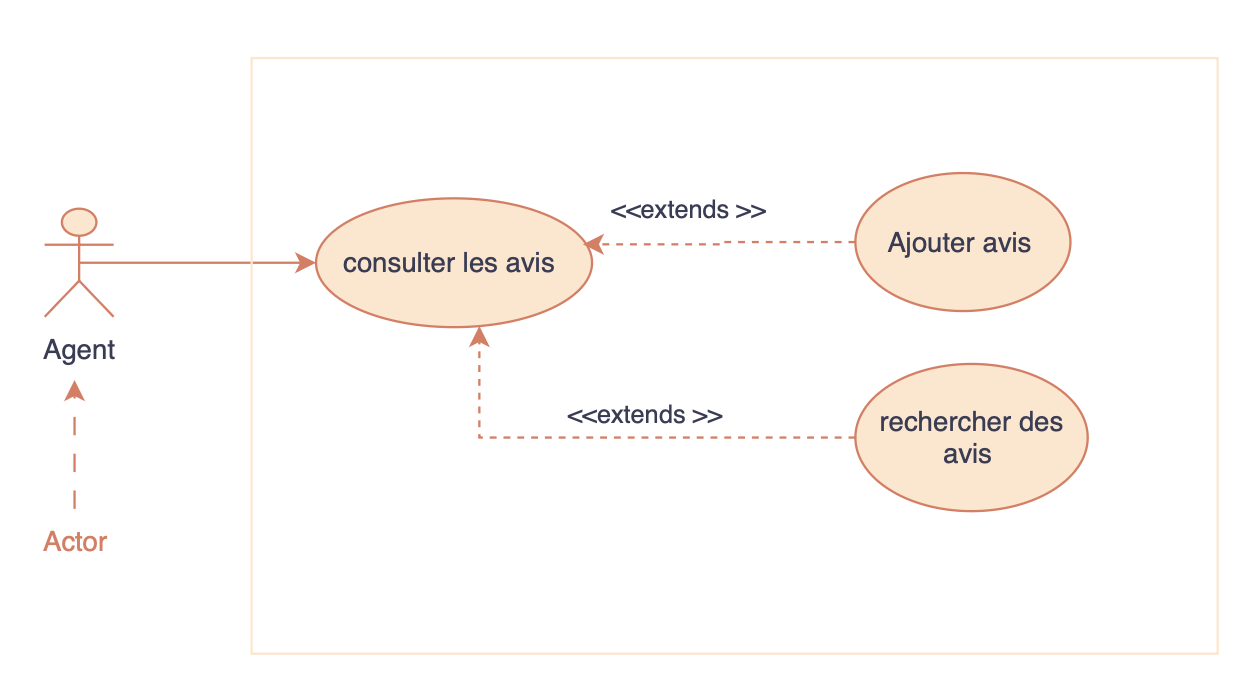
\includegraphics[width=0.8\textwidth]{images/diagramme/casUtilisation1.png}
            \caption{Diagramme de cas d'utilisation}
        \end{figure}
        \vspace{7cm}

        \subsubsection{2.2.2\hspace{2em}Diagramme d'activité}
        Le diagramme d'activité suivant, permet d'illustrer les différents choix que l'utilisateur pourra faire. Ce diagramme nous montre les actions des différents boutons.
        \medskip

        \begin{figure}[h!]
            \centering
            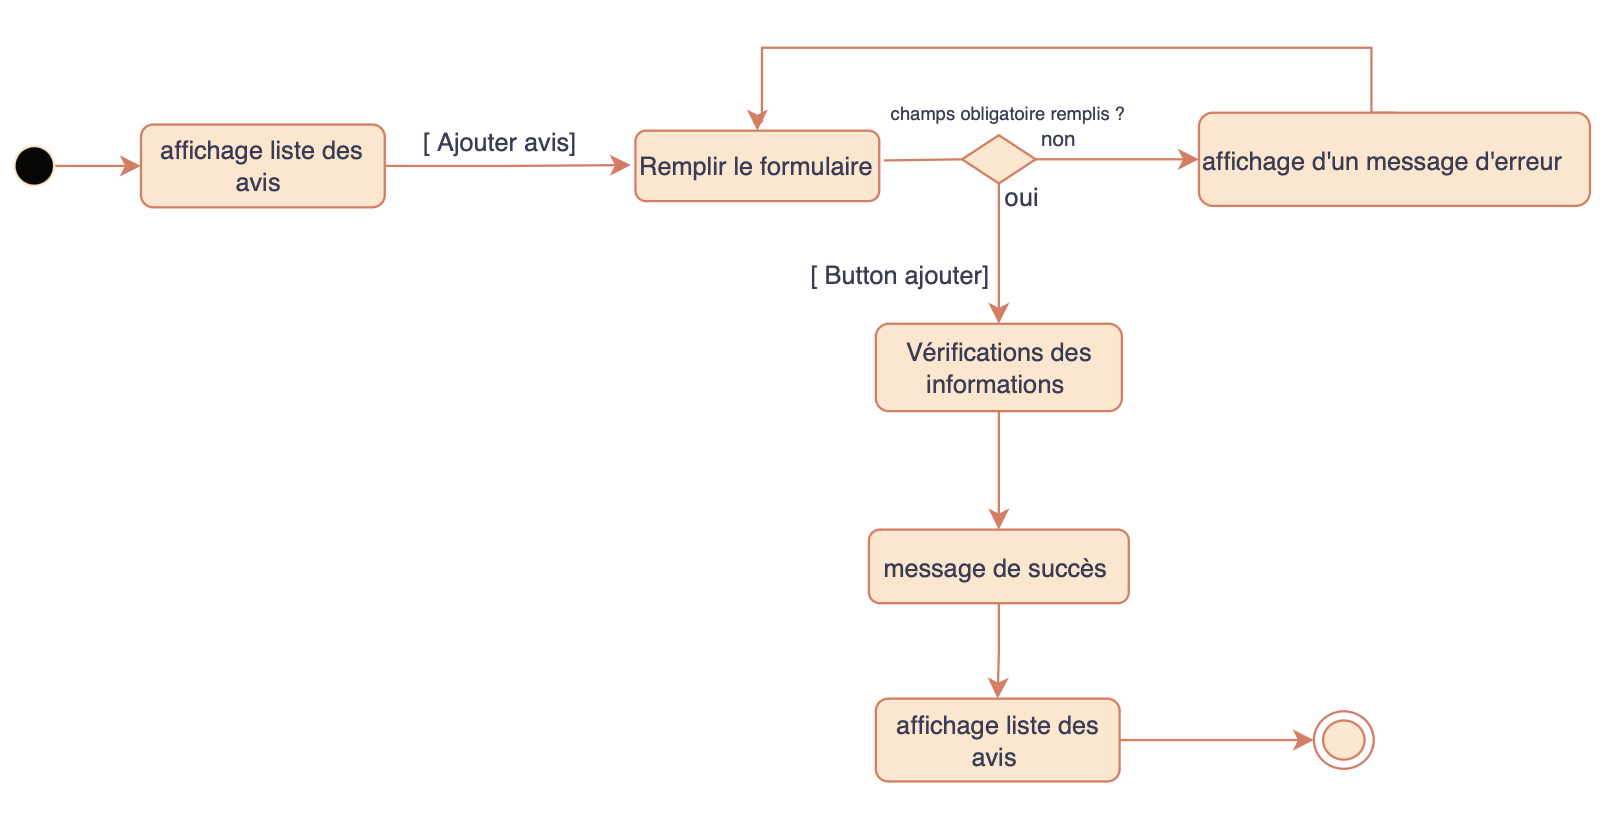
\includegraphics[width=0.9\textwidth]{images/diagramme/activite.png}
            \caption{Diagramme d'activité du cas d'utilisation ajouter avis}
        \end{figure}
        \medskip

        \subsubsection{2.2.3\hspace{2em}Diagramme de classe}
        Après réflexion avec mon tuteur sur le modèle de données le plus adapté pour représenter les données, nous sommes arrivés au diagramme de classe suivant :
        \vspace{3cm}

        \begin{figure}[h!]
            \centering
            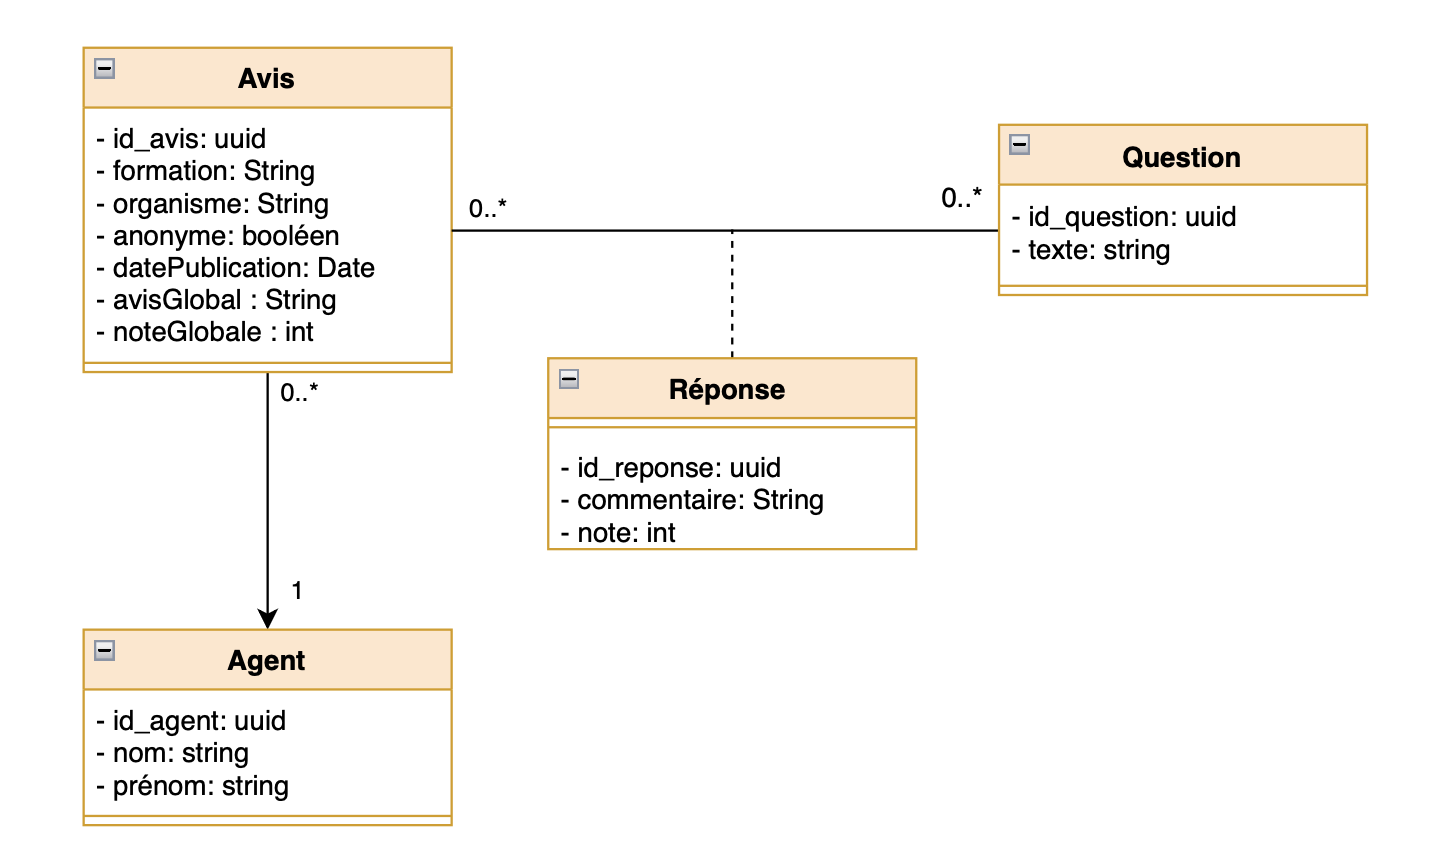
\includegraphics[width=0.9\textwidth]{images/diagramme/cllasse.png}
            \caption{Diagramme de classe UML}
        \end{figure}
        \medskip
    
        \subsubsection{2.2.4\hspace{2em}Choix techniques et implémentation}
        Dans un premier temps, nous avons utilisé une base de données H2 avec Spring Boot. 
        H2 est une base de données rapide et légère qui offre la possibilité d'une persistance 
        dans un fichier.\medskip
        
        Lors du développement du service backend, une bonne pratique pour travailler avec les 
        bases de données est de ne pas utiliser la génération et la mise à jour automatique du 
        schéma avec Hibernate/JPA, mais plutôt utiliser Flyway, qui est un outil de migration 
        de base de données qui met à jour la base de données de manière cohérente et contrôlée.\vspace{0.5cm}

        Aprés avoir défini et visualisé notre modèle de données à l'aide des diagrammes UML, 
        nous avons commencé par créer les classes entités définies dans le diagramme de classes.
        \vspace{11cm}

        \begin{figure}[h!]
            \centering
            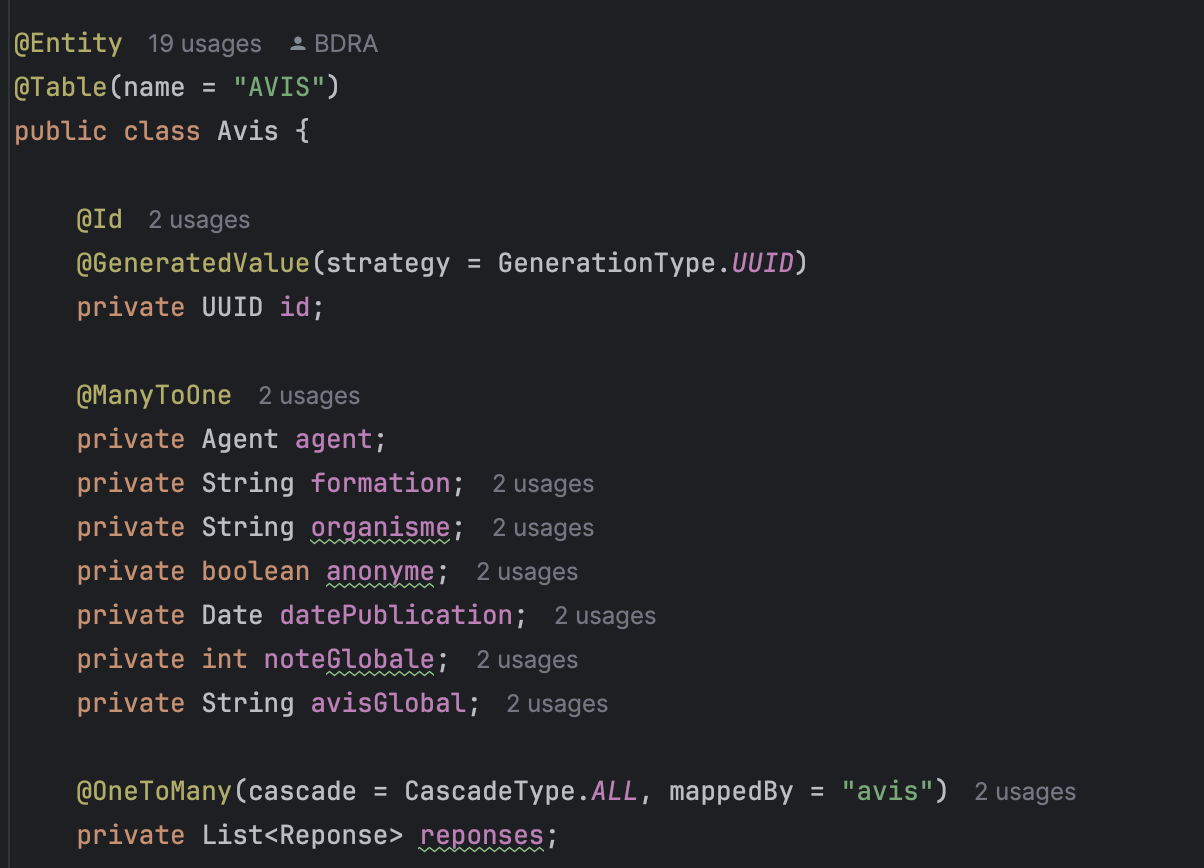
\includegraphics[width=0.8\textwidth]{images/code/avisEntity.png}
            \caption{Exemple de classe model de l'application}
        \end{figure}\medskip

        Les différentes classes Java comportent plusieurs notations :
        \medskip
        
        \textbf{@Entity}: permet à Hibernate/JPA de les considérer comme des ORM qui transfère les données entre l'application et la base de données.
        \medskip

        \textbf{@Table}: permet de mapper l'entité en table physique dans la base de données.
        \medskip

        \textbf{@Id}: permet d'identifier un attribut de la classe comme clé primaire de la table.
        \medskip

        \textbf{@GeneratedValue(strategy = GenerationType.UUID)}: est utilisée pour spécifier la stratégie de génération de clé primaire. L'attribut 'strategy' détermine comment la clé primaire est générée, dans ce cas elle est sous forme de UUID.\medskip

        \textbf{@Column}: permet de mapper un attribut de la classe à une colonne de la table.
        \medskip

        \textbf{@ManyToOne, @OneToMany}: permet de gérer les associations (*, 1) et (1, *) entre deux entités.
        \vspace{1cm}

        Pour transfèrer nos données entre les différentes couches de notre application de manière optimisée, nous avons adopté l'utilisation des classes DTO (Data Transfer Object).
        Les classes DTO sont des objets simples utilisés pour tranférer uniquement les données nécessaires.\medskip

        \begin{figure}[h!]
            \centering
            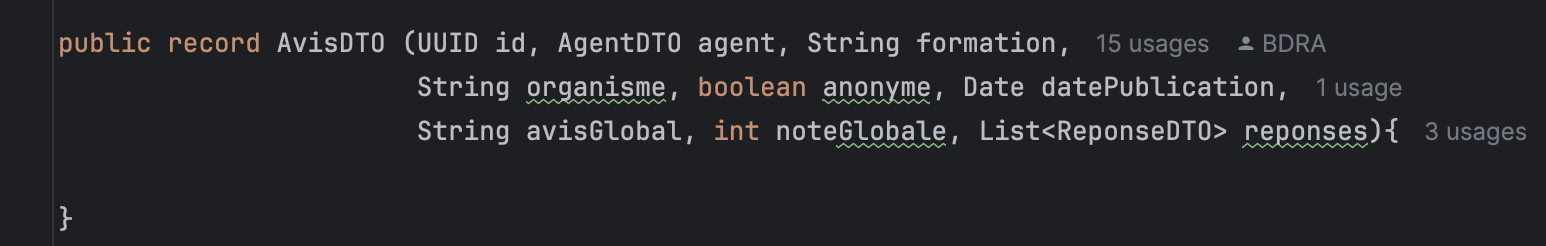
\includegraphics[width=0.8\textwidth]{images/code/AvisDTO.png}
            \caption{Exemple de classe DTO de l'application}
        \end{figure}\vspace{1cm}


        Pour nos classes Repository (DAO) nous avons utilisé Spring Data JPA pour gérer l'accès aux données. Cette classe utilise l'interface JpaRepository, pour effectuer des opérations de base telles que sauvegarder, trouver, mettre à jour et supprimer des données sans avoir à écrire beaucoup de code. 
        Cela réduit le besoin d'écrire des requêtes SQL manuellement, car Spring Data JPA génère automatiquement les requêtes nécessaires.\medskip

        \begin{figure}[h!]
            \centering
            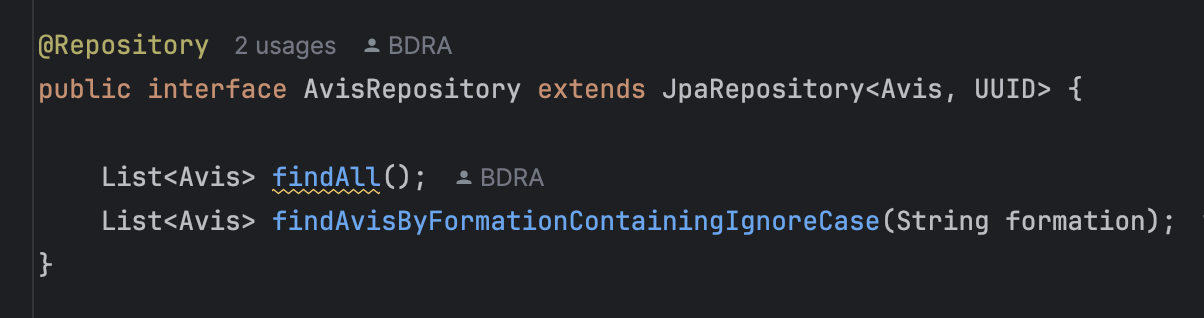
\includegraphics[width=0.8\textwidth]{images/code/DAOAvis.png}
            \caption{Exemple de classe Repository de l'application}
        \end{figure}
        \vspace{1cm}

        Les classes Services de notre application sont celles qui font appel aux DAO, dans le but de récupérer les données, les traiter et les faire transiter aux 'Controller'.
        \medskip

        \begin{figure}[h!]
            \centering
            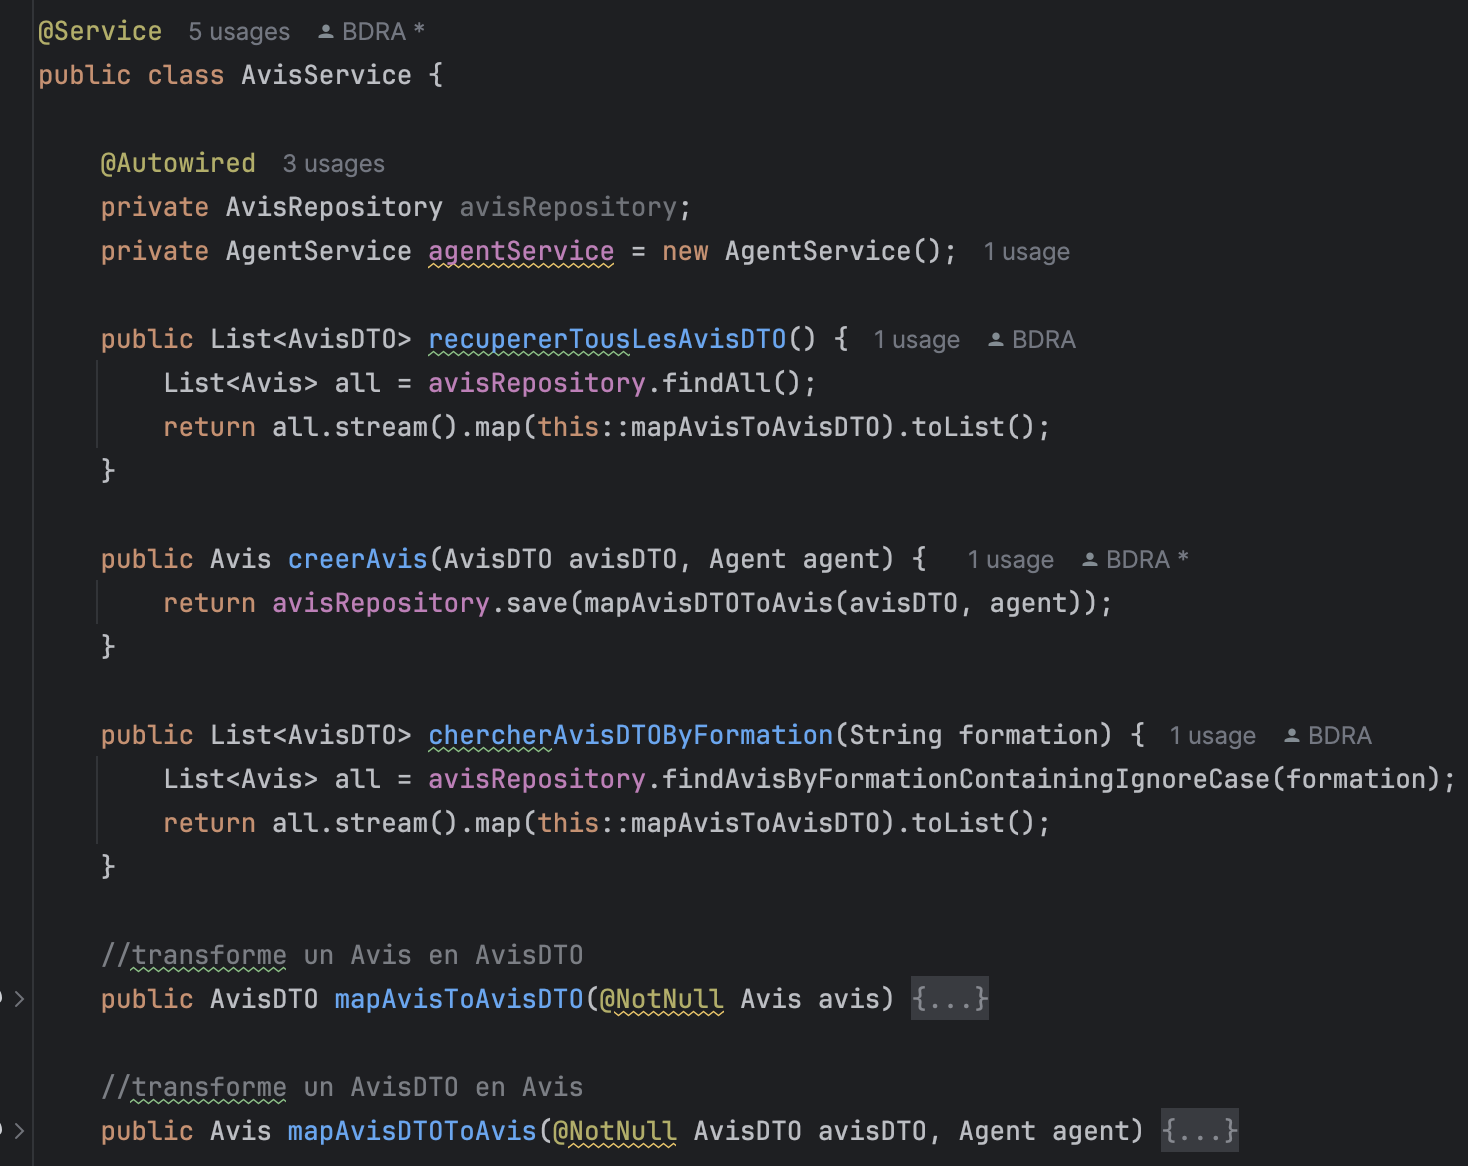
\includegraphics[width=0.8\textwidth]{images/code/avisService.png}
            \caption{Exemple de classe Service de l'application}
        \end{figure}\medskip

        Les différentes classes comportent plusieurs notations :
        \medskip

        \textbf{@Service}: permet d'indiquer que cette classe contient la logique métier et permet à Spring de détecter automatiquement cette classe.
        \medskip

        \textbf{@Autowired}: permet à Spring d'injecter une instance d'une classe existante dans la classe service. Cela permet au service d'utiliser cette instance pour accéder aux données.
        \vspace{1cm}

        Les classes Contrôleurs de notre application sont responsables de gérer les requêtes HTTP entrantes, d'appeler les services appropriés, et de renvoyer les réponses. Les contrôleurs définissent les points d'accès de l'API et orchestrent les interactions entre les utilisateurs et le système.
        \medskip

        \begin{figure}[h!]
            \centering
            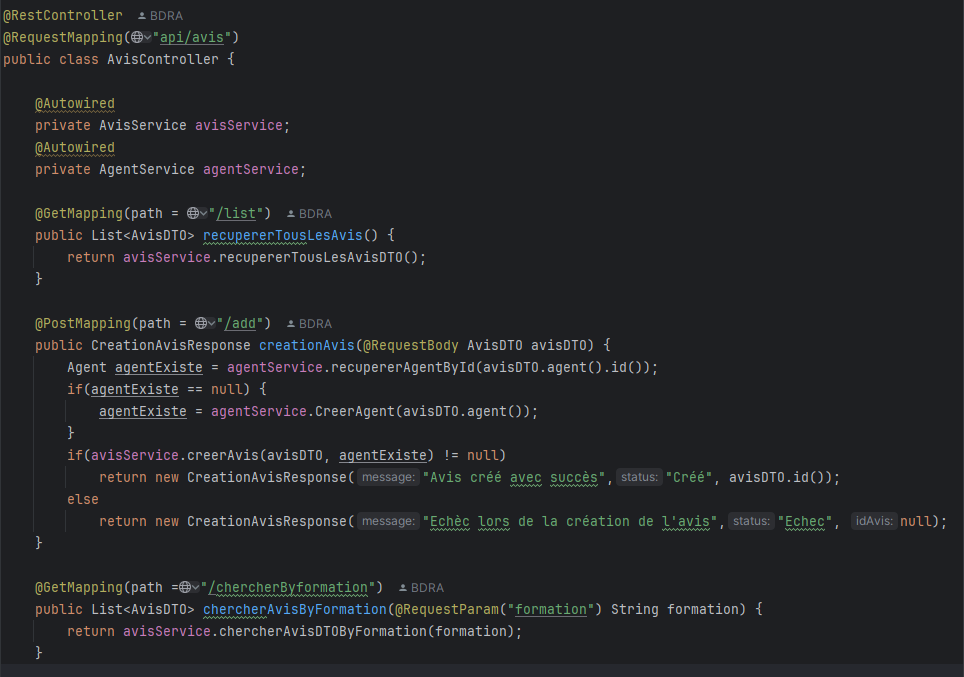
\includegraphics[width=0.8\textwidth]{images/code/controlleurAvis.PNG}
            \caption{Exemple de classe Controller de l'application}
        \end{figure}
        \medskip

        Les principales annotations utilisées dans les classes contrôleurs :
        \medskip

        \textbf{@RestController}: indique que la classe est un contrôleur ou chaque méthode de gestion de requêtes renvoie un objet directement en format JSON ou XML, plutôt que de renvoyer une vue.
        \medskip

        \textbf{@RequestMapping}: permet de mapper les requêtes HTTP à des méthodes spécifiques dans un contrôleur. Elle peut être appliqué au niveau de la classe et au niveau des méthodes pour définir des URL de base et des URL spécifiques.\\
        Dans cet exemple toutes les requêtes HTTP commençant par '/api/avis' seront dirigées vers les méthodes de ce contrôleur.
        \medskip

        \textbf{@GetMapping}: spécification de '@RequestMapping' pour les requêtes HTTP GET. Elle est utilisée pour définir les points d'accès qui répondent aux requêtes GET.
        \medskip

        \textbf{@PostMapping}: spécification de '@RequestMapping' pour les requêtes HTTP POST. Elle est utilisée pour définir les points d'accès qui répondent aux requêtes POST.
        \medskip

        
